\documentclass[11pt,a4paper]{article}
\usepackage{fontspec}
\usepackage{polyglossia}
\setdefaultlanguage{russian}
\setotherlanguage{english}
\setmainfont{Liberation Serif}
\setsansfont{DejaVu Sans}
\setmonofont{DejaVu Sans Mono}[Scale=0.85]
\usepackage{amsmath,amssymb,amsthm}
\usepackage{xcolor}
\usepackage[margin=2.3cm]{geometry}
\usepackage{graphicx,booktabs,array,longtable}
\usepackage[font=small,labelfont=bf]{caption}
\usepackage{enumitem}
\usepackage[section]{placeins}
\usepackage[colorlinks=true,linkcolor=blue!50!black,citecolor=blue!50!black,urlcolor=blue!50!black]{hyperref}
\setlist{nosep,leftmargin=1.4em}
\linespread{1.08}
\emergencystretch=1.5em

\theoremstyle{plain}
\newtheorem{theorem}{Теорема}
\newtheorem{lemma}{Лемма}
\newtheorem{proposition}{Предложение}
\newtheorem{corollary}{Следствие}
\newtheorem{conjecture}{Гипотеза}
\theoremstyle{definition}
\newtheorem{definition}{Определение}
\newtheorem{remark}{Замечание}
\renewcommand{\proofname}{Доказательство}

\newcommand{\G}{\Gamma}
\newcommand{\dd}{\,\mathrm{d}}

\title{Дробные деревья Вольтерры и упрощающие условия\\ для явных методов Рунге--Кутты дробного порядка}
\author{Д.\,А.~Приказчиков\\[2pt]
\small Московский физико-технический институт (национальный исследовательский университет),\\
\small г.~Долгопрудный, Московская обл., 141701, Россия\\
\small E-mail: \texttt{prikazchikov.da@phystech.edu}}
\date{Черновик от 17 октября 2026 г.}

\begin{document}
\maketitle

\begin{abstract}
Работа продолжает исследование явных одношаговых методов типа Рунге--Кутты для задачи Коши с дробной производной Капуто порядка $\alpha\in(0,1)$, записанной в форме уравнения Вольтерры. Получено полное разложение локальной ошибки таких методов в ряд по степеням $h^{K+N\alpha}$. Члены ряда индексируются корневыми деревьями с вершинами двух типов: листья отвечают дифференцированию по времени и имеют вес $1$, внутренние вершины отвечают интегрированию с дробным ядром и имеют вес $\alpha$. Веса деревьев выражаются через таблицу Бутчера и квадратурные дефекты стадий, а элементарные дифференциалы~--- через полные производные правой части вдоль решения. Доказана теорема о разложении с оценкой остатка. Показано, что во внутренней точке сетки эти производные можно задавать независимо, откуда следует \emph{необходимость} условий порядка~--- звено, требующееся для доказательства барьеров. Найдено число условий на каждом уровне и описан скалярный случай. Введён дробный аналог упрощающих условий Бутчера: точность стадий на линейной функции с дробным ядром и \guillemotleft выключение\guillemotright\ второй стадии. При пяти стадиях эти условия сводят систему из шестнадцати условий порядка к семи уравнениям на шесть неизвестных, у которой численно найдено ровно два семейства решений. С их помощью построены пятистадийные методы с показателем локальной ошибки $\min(1+5\alpha,\,4+\alpha)$ при $\alpha\in[0.5;\,0.95]$, коэффициентами порядка единиц и узлами в пределах шага с небольшим выходом за его конец. Этим уточняется гипотеза о барьере для пяти стадий, выдвинутая ранее: вместо ветви $3+2\alpha$ численные результаты указывают на ветвь $4+\alpha$, которая при $\alpha\to1$ переходит в классическое ограничение порядка. Показатели построенных методов подтверждены прямым измерением локальной ошибки в арифметике повышенной точности. Код и данные открыты.

\medskip\noindent\textbf{Ключевые слова:} дробные дифференциальные уравнения, производная Капуто, методы Рунге--Кутты, уравнения Вольтерры, корневые деревья, условия порядка, упрощающие условия, барьеры Бутчера.
\end{abstract}

\section{Введение}

Явные одношаговые методы для дробно-дифференциальных уравнений привлекательны в задачах наследственной механики: при локализации интегродифференциальных уравнений вязкоупругости с ядром Работнова переменные памяти среды удовлетворяют дробно-дифференциальным уравнениям по времени~\cite{PP2026zhvm,Prik2026de}, и метод интегрирования по времени должен легко встраиваться в явную схему по пространству. В работе~\cite{PrikBarriers} для задачи Коши
\begin{equation}\label{eq:fde}
{}^{C}\!D^{\alpha}_{0}y(t)=f\bigl(t,y(t)\bigr),\qquad y(0)=y_0,\qquad 0<\alpha<1,
\end{equation}
были рассмотрены явные методы в форме Вольтерры (класс Пуазе~\cite{Pouzet1960} и Любича~\cite{Lubich1983}), получено явное представление младших членов их локальной ошибки и доказан дробный аналог первого барьера Бутчера: наилучший показатель локальной ошибки равен $1+2\alpha$ при двух стадиях, $\max(2+\alpha,\,1+3\alpha)$ при трёх и не превосходит $\max(2+2\alpha,\,1+4\alpha)$ при четырёх. Для пяти стадий там же на основании численного поиска была высказана гипотеза о барьере $\max\bigl(2+3\alpha,\,\min(1+5\alpha,3+2\alpha)\bigr)$.

Дальнейшее продвижение упирается в два обстоятельства. Во-первых, представления младших членов недостаточно: при пяти стадиях существенны члены, которые в~\cite{PrikBarriers} входили в остаток. Во-вторых, численный поиск методов, удовлетворяющих большому числу условий порядка, оказывается ненадёжным: как показано ниже, решения систем условий при $s=5$ вырождены и обладают большими коэффициентами, так что случайный поиск их не находит, и отрицательный результат такого поиска ещё не свидетельствует о несуществовании.

Настоящая работа посвящена обоим вопросам. Опишем, что здесь известно и что ново. Теория методов Рунге--Кутты для уравнений Вольтерры восходит к работе Брунера, Хайрера и Нёрсетта~\cite{BHN1982}; Любич~\cite{Lubich1983} распространил её на ядра со слабой особенностью, ввёл деревья Вольтерры с весом $\mathrm{fin}+(1+a)\,\mathrm{int}$ и доказал \emph{достаточность} соответствующих условий порядка; Гаррапа~\cite{Garrappa2010} предложил алгоритм автоматической генерации условий. Классические упрощающие условия Бутчера~\cite{Butcher1964,Butcher2016,HNW1993} позволяют свести условия высокого порядка к небольшой системе; для пятого и шестого порядков используется приём, при котором вторая стадия исключается из всех условий, кроме условий на её собственный столбец. Новыми являются: для уравнения~\eqref{eq:fde} в форме Вольтерры~--- явное представление локальной ошибки как тождества с элементарными дифференциалами, выраженными через полные производные правой части вдоль решения, и с оценкой остатка (теорема~\ref{thm:bseries}); лемма о свободе этих производных и вытекающая из неё необходимость условий порядка (теорема~\ref{thm:necessity}); подсчёт числа условий и обрезание по стадийной высоте; дробные упрощающие условия и сведение задачи для пяти стадий к системе из семи уравнений (теорема~\ref{thm:reduced}); численное описание её решений и построенные с их помощью методы. Статусы результатов указываются по ходу изложения: теоремы доказаны, численные утверждения названы таковыми, гипотезы сформулированы явно.

\section{Математическая постановка и теоремы}

\subsection{Класс методов}

Обозначения совпадают с~\cite{PrikBarriers}. Пусть $t_n=nh$. Решение задачи~\eqref{eq:fde} при $t>t_n$ представляется в виде
\begin{equation}\label{eq:split}
y(t)=\Phi_n(t)+\frac{1}{\G(\alpha)}\int_{t_n}^{t}(t-s)^{\alpha-1}g(s)\dd s ,\qquad g(t)=f\bigl(t,y(t)\bigr),
\end{equation}
где лаг-член $\Phi_n$ содержит интеграл по пройденной предыстории $[0,t_n]$. Явный $s$-стадийный метод имеет вид
\begin{equation}\label{eq:method}
Y_i=\Phi_n(t_n+c_ih)+h^{\alpha}\sum_{j<i}a_{ij}F_j,\qquad F_j=f(t_n+c_jh,Y_j),\qquad
y_{n+1}=\Phi_n(t_{n+1})+h^{\alpha}\sum_{j=1}^{s}b_jF_j ,
\end{equation}
причём
\begin{equation}\label{eq:rowsum}
c_1=0,\qquad 0\le c_i\le\hat c,\qquad \sum_{j<i}a_{ij}=\frac{c_i^{\alpha}}{\G(\alpha+1)}\quad(i=2,\dots,s),
\end{equation}
т.\,е. каждая стадия точно интегрирует постоянные; в расчётах $\hat c=1.5$. Локальной ошибкой называется $\delta_n=y_{n+1}-y(t_{n+1})$ при точном лаг-члене, показателем метода~--- наибольшее $q$, при котором $\delta_n=O(h^q)$ для всех гладких $f$ (для систем любой размерности), а через $q(s,\alpha)$ обозначается верхняя грань показателей явных $s$-стадийных методов. Значения интегралов от мономов даёт формула
\begin{equation}\label{eq:beta}
\frac{1}{\G(\alpha)}\int_0^{c}(c-\theta)^{\alpha-1}\theta^k\dd\theta=\gamma_k\,c^{k+\alpha},\qquad \gamma_k=\frac{k!}{\G(k+\alpha+1)} .
\end{equation}
Квадратурные дефекты стадий и выхода~--- это
\[
d_k=Ac^k-\gamma_k\,c^{\,k+\alpha}\in\mathbb R^s,\qquad D_k=b^{\top}c^k-\gamma_k ;
\]
по~\eqref{eq:rowsum} $d_0=0$, а первая компонента любого $d_k$ равна нулю. Степени векторов и произведения векторов, обозначаемые точкой, понимаются покомпонентно, $C=\mathrm{diag}(c)$.

% Раздел статьи 2: общая структура локальной ошибки. Черновик 16.10.2026.
\subsection{Деревья и элементарные дифференциалы}\label{sec:trees}

Напомним, что в~\cite{PrikBarriers} было получено явное представление младших членов локальной ошибки (предложение~1 там), а остальные члены объединялись в остаток $\rho_n=O(h^{\min(3+\alpha,\,2+3\alpha)})$. Опишем полное разложение.

Основную роль в разложении играют полные производные правой части вдоль решения в точке $t_n$:
\begin{equation}\label{eq:atoms}
D_{r,k}=\frac{\dd^k}{\dd t^k}\,\partial_y^rf\bigl(t,y(t)\bigr)\Big|_{t=t_n},\qquad r,k\ge0,
\end{equation}
так что $D_{0,k}=g_k$, $D_{1,0}=J$, $D_{1,1}=J'$; при $r\ge1$ величина $D_{r,k}$ является симметрическим $r$-линейным отображением. Будем называть их \emph{атомами}. В отличие от классической теории, где элементарные дифференциалы строятся из частных производных $f$, здесь удобнее полные производные: значения $y'(t_n),y''(t_n),\dots$ во внутренней точке определяются всей предысторией, а не значением $f$ в этой точке, и атомы оказываются независимыми параметрами задачи (лемма~\ref{lem:free}).

Индексирующими объектами служат обычные корневые деревья~--- те же, что и в теории Бутчера~\cite{Butcher2016,HNW1993}, но с иной ролью вершин. Вершины дерева $T$ разделим на два типа. \emph{Листья} будем называть \emph{временны\'ми} вершинами: каждый лист отвечает одному дифференцированию по времени и приносит множитель $h$. Все остальные вершины, включая корень, будем называть \emph{стадийными}: каждая стадийная вершина отвечает одному интегрированию с ядром $(t-s)^{\alpha-1}/\G(\alpha)$, т.\,е. одному множителю $h^{\alpha}$ в~\eqref{eq:method}. Дерево из одной вершины состоит из одного корня, который считается стадийным. Обозначим через $N(T)$ число стадийных вершин, через $K(T)$~--- число листьев и положим
\begin{equation}\label{eq:order}
|T|=N(T)\,\alpha+K(T).
\end{equation}
Для стадийной вершины $v$ через $k_v$ обозначим число её детей-листьев, через $r_v$~--- число детей-стадий. Стадийную вершину с $r_v=0$ назовём \emph{висячей}; поскольку она не является листом, у неё $k_v\ge1$ (кроме случая дерева из одной вершины).

\begin{definition}\label{def:F}
Элементарный дифференциал дерева определяется рекурсией по корню $\rho$:
\[
F(T)=D_{r_\rho,k_\rho}\bigl(F(T_1),\dots,F(T_{r_\rho})\bigr),
\]
где $T_1,\dots,T_{r_\rho}$~--- поддеревья с корнями в детях-стадиях корня $\rho$; для висячей вершины $F=g_{k_\rho}$, для дерева из одной вершины $F=g_0$. Коэффициент симметрии $\sigma(T)$~--- обычный коэффициент Бутчера: $\sigma(\bullet)=1$, $\sigma(T)=\prod_i\mu_i!\,\sigma(T_i)^{\mu_i}$, где $\mu_i$~--- кратности попарно различных поддеревьев корня (одинаковые листья учитываются, что даёт множитель $k_\rho!$).
\end{definition}

Например, дереву, у которого корень имеет одного ребёнка-стадию, а тот~--- два листа, отвечают $F=Jg_2$, $|T|=2+2\alpha$, $\sigma=2$; это член $C_1$ работы~\cite{PrikBarriers}. Дереву с корнем, имеющим один лист и одного ребёнка-стадию с одним листом, отвечают $F=J'g_1$ и тот же показатель $2+2\alpha$; это член $C_2$. Цепочка из $m+1$ стадийных вершин, последняя из которых имеет один лист, даёт $F=J^mg_1$ и $|T|=1+(m+1)\alpha$~--- цепочку $B_m$.

\paragraph{Веса.} Пусть задана таблица $(c,A,b)$ явного метода. Каждой некорневой стадийной вершине $v$ сопоставим вектор $\varphi(v)\in\mathbb R^s$ рекурсией снизу вверх:
\begin{equation}\label{eq:phi}
\varphi(v)=\begin{cases}
d_{k_v}=Ac^{k_v}-\gamma_{k_v}\,c^{\,k_v+\alpha}, & r_v=0,\\[1mm]
A\Bigl(c^{k_v}\cdot\varphi(u_1)\cdots\varphi(u_{r_v})\Bigr), & r_v\ge1,
\end{cases}
\qquad \gamma_k=\frac{k!}{\G(k+\alpha+1)},
\end{equation}
где $u_1,\dots,u_{r_v}$~--- дети-стадии вершины $v$, а точка обозначает покомпонентное произведение. Вес дерева определяется корнем:
\begin{equation}\label{eq:Psi}
\Psi(T)=\begin{cases}
D_{k_\rho}=b^{\top}c^{k_\rho}-\gamma_{k_\rho}, & r_\rho=0,\\[1mm]
b^{\top}\Bigl(c^{k_\rho}\cdot\varphi(u_1)\cdots\varphi(u_{r_\rho})\Bigr), & r_\rho\ge1.
\end{cases}
\end{equation}
Квадратурные дефекты $d_k$, $D_k$ здесь те же, что и в~\cite{PrikBarriers}, с точностью до множителя: $\gamma_k$~--- значение интеграла~\eqref{eq:beta} при $c=1$.

Отметим характерную особенность весов~\eqref{eq:phi}, \eqref{eq:Psi}: точное решение входит в них \emph{только через висячие вершины}, т.\,е. через дефекты $d_k$ и $D_k$, а каждая внутренняя вершина несёт чисто численный оператор $A\,\mathrm{diag}(c^{k})$. Причина в том, что разложение правой части в каждой стадии ведётся вокруг точного решения; сравнивать с точным значением приходится лишь квадратуру гладкой функции $g$ на текущем шаге, а не результат применения $f$ к неточным стадиям. Раскрывая произведения дефектов, получаем представление веса через бета-интегралы:
\begin{equation}\label{eq:Psi-beta}
\Psi(T)=\sum_{S\subseteq\mathcal L(T)}(-1)^{|S|}\Bigl(\prod_{v\in S}\gamma_{k_v}\Bigr)\,\Phi_S(T),
\end{equation}
где $\mathcal L(T)$~--- множество висячих вершин, а $\Phi_S(T)$~--- обычный численный вес дерева, в котором для $v\in S$ множитель $Ac^{k_v}$ заменён на $c^{k_v+\alpha}$ (а для висячего корня $b^{\top}c^{k}$~--- на единицу). При $\alpha=1$ имеем $\gamma_kc^{k+1}=c^{k+1}/(k+1)$, и условия $\Psi(T)=0$ треугольным преобразованием сводятся к классическим условиям Бутчера $\Phi(T)=1/\gamma(T)$. При $\alpha<1$ дробные степени $c^{k+\alpha}$, попадающие под действие матрицы $A$, через другие условия не выражаются, и такой редукции нет: именно поэтому каждое дерево даёт отдельное условие.

\paragraph{Связь с деревьями Вольтерры.} Правило~\eqref{eq:order} совпадает с правилом $\mathrm{fin}(t)+(1+a)\,\mathrm{int}(t)$ для деревьев Вольтерры Любича~\cite{Lubich1983}, где $a=\alpha-1$~--- показатель ядра $(x-s)^{a}$, а корень также считается внутренней вершиной. Для ядра общего вида $(x-s)^aK(x,s,y)$ концевые вершины деревьев Любича могут нести дополнительный индекс, отвечающий производной ядра по первому аргументу; для уравнения~\eqref{eq:fde} функция $K=f(s,y)/\G(\alpha)$ от $x$ не зависит, такие вершины не возникают, и индексирующее множество сводится к обычным корневым деревьям. Веса Любича также определены рекурсивно, с дефектами квадратуры в концевых вершинах, и теорема~6 работы~\cite{Lubich1983} утверждает \emph{достаточность} условий $\varphi(t)=0$ для заданного порядка локальной ошибки. Алгоритм автоматической генерации условий для уравнений Вольтерры со слабосингулярным ядром предложен Гаррапой~\cite{Garrappa2010}. Новыми в настоящем разделе являются: представление локальной ошибки как тождества с явными элементарными дифференциалами~\eqref{eq:atoms} и оценкой остатка (теорема~\ref{thm:bseries}), лемма о свободе атомов и вытекающая из неё \emph{необходимость} условий (теорема~\ref{thm:necessity})~--- именно она требуется для доказательства барьеров,~--- а также подсчёт числа условий, обрезание по стадийной высоте и описание скалярного случая.

\subsection{Разложение локальной ошибки}

Обозначим через $\mathcal E=\{N\alpha+K\}$ множество показателей~\eqref{eq:order} всех деревьев; оно дискретно, и для любого $P>0$ определено $P^{+}=\min\{x\in\mathcal E:\ x>P\}$.

\begin{theorem}[разложение локальной ошибки]\label{thm:bseries}
Пусть $P>0$, $M=\lfloor P\rfloor+1$, $f\in C^{M}$ в окрестности дуги $\{(t,y(t)):\,t\in[t_n,t_n+\hat ch]\}$, $y\in C^{M}[t_n,t_n+\hat ch]$. Тогда для метода~\eqref{eq:method}, \eqref{eq:rowsum}
\begin{equation}\label{eq:bseries}
\delta_n=\sum_{T:\ |T|\le P}\frac{h^{|T|}}{\sigma(T)}\,\Psi(T)\,F(T)+\rho_n,\qquad |\rho_n|\le K_P\,h^{P^{+}},
\end{equation}
а ошибки стадий $e_i=Y_i-y(t_n+c_ih)$ представляются в виде
\begin{equation}\label{eq:stage-series}
e_i=\sum_{T\ne\bullet:\ |T|\le P}\frac{h^{|T|}}{\sigma(T)}\,\varphi_i(T)\,F(T)+O\bigl(h^{P^{+}}\bigr),
\end{equation}
где $\varphi(T)$~--- вектор~\eqref{eq:phi}, вычисленный для корня дерева $T$. Постоянная $K_P$ зависит от норм производных $f$ порядка не выше $M$ в окрестности дуги, норм $y^{(j)}$, $j\le M$, от $\max|a_{ij}|$, $\max|b_i|$ и от $\hat c$, но не от $h$; при $y\in C^{M}[t_*,T+\hat ch_0]$, $t_*>0$, она равномерна по шагам с $t_n\ge t_*$, $h\le h_0$.
\end{theorem}

Предложение~1 работы~\cite{PrikBarriers} есть частный случай теоремы~\ref{thm:bseries} при $P<\min(3+\alpha,2+3\alpha)$: деревья с $|T|$ ниже этого значения~--- это в точности $D_0,D_1,D_2$, цепочки $B_m$ и два дерева $C_1,C_2$.

Доказательству предпошлём комбинаторное наблюдение. Каждое дерево с корнем, имеющим $k$ листьев и детей-стадий $T_1,\dots,T_r$, будем записывать как $[\,k;\,T_1,\dots,T_r\,]$.

\begin{lemma}[подстановка рядов]\label{lem:subst}
Пусть $\varepsilon=\sum_{T\in\mathcal S}\frac{h^{|T|}}{\sigma(T)}x(T)F(T)$~--- конечная сумма по множеству $\mathcal S$ деревьев с числовыми коэффициентами $x(T)$. Тогда для $r\ge1$, $k\ge0$
\[
\frac{1}{k!\,r!}\,\tau^k\,D_{r,k}\bigl(\varepsilon,\dots,\varepsilon\bigr)
=\sum_{T_1,\dots,T_r\in\mathcal S}{}^{'}\ \frac{h^{|U|-\alpha-k}\,\tau^k}{\sigma(U)}\,x(T_1)\cdots x(T_r)\,F(U),\qquad U=[\,k;\,T_1,\dots,T_r\,],
\]
где штрих означает суммирование по неупорядоченным наборам $\{T_1,\dots,T_r\}$ (мультимножествам).
\end{lemma}
\begin{proof}
Раскрывая полилинейное выражение, получаем сумму по упорядоченным наборам $(T_1,\dots,T_r)$. Мультимножество с кратностями $\mu_i$ встречается $r!/\prod\mu_i!$ раз, и в силу симметрии $D_{r,k}$ все эти слагаемые равны $D_{r,k}(F(T_1),\dots,F(T_r))=F(U)$. Показатель $h$ равен $\sum|T_l|=|U|-\alpha-k$, а коэффициент~--- $\frac{1}{k!\prod\mu_i!\prod\sigma(T_l)}=\frac{1}{\sigma(U)}$ по определению~\ref{def:F}.
\end{proof}

\begin{proof}[Доказательство теоремы~\ref{thm:bseries}]
\emph{Шаг 1: точное соотношение для ошибок стадий.} Вычитая из~\eqref{eq:method} равенство~\eqref{eq:split} при $t=t_n+c_ih$, получаем
\begin{equation}\label{eq:err-exact}
e_i=h^{\alpha}\Bigl[\sum_ja_{ij}\,g(t_n+c_jh)-\frac{1}{\G(\alpha)}\int_0^{c_i}(c_i-\theta)^{\alpha-1}g(t_n+\theta h)\dd\theta\Bigr]
+h^{\alpha}\sum_{j<i}a_{ij}\bigl[f(t_j,y(t_j)+e_j)-g(t_j)\bigr],
\end{equation}
$t_j=t_n+c_jh$, и то же для $\delta_n$ с заменой $a_{ij}$ на $b_j$ и $c_i$ на $1$.

\emph{Шаг 2: квадратурная часть.} По формуле Тейлора $g(t_n+\theta h)=\sum_{k<M}g_k\frac{(\theta h)^k}{k!}+O(h^M)$ равномерно по $\theta\in[0,\hat c]$; с учётом~\eqref{eq:beta} первая скобка в~\eqref{eq:err-exact} равна
\[
\sum_{k<M}\frac{h^k}{k!}\,(d_k)_i\,g_k+O(h^{M}),
\]
причём $d_0=0$ по~\eqref{eq:rowsum}. Слагаемое с номером $k$ умножается на $h^{\alpha}$ и даёт член $h^{k+\alpha}\frac{(d_k)_i}{k!}g_k$ ряда~\eqref{eq:stage-series}, отвечающий висячему дереву $[\,k;\,]$ с $\sigma=k!$. Остаток имеет порядок $h^{M+\alpha}$; поскольку $M+\alpha=|[\,M;\,]|\in\mathcal E$ и $M+\alpha>P$, имеем $M+\alpha\ge P^{+}$.

\emph{Шаг 3: индукция по номеру стадии.} Метод явный, поэтому $e_1=0$ (первая строка $A$ нулевая, $c_1=0$), а $e_i$ выражается через $e_1,\dots,e_{i-1}$. Предположим, что~\eqref{eq:stage-series} доказано для всех $j<i$. В частности, $e_j=O(h^{1+\alpha})$, так как наименьший показатель некорневого дерева равен $1+\alpha$. Положим $R=\lfloor(P-\alpha)/(1+\alpha)\rfloor$. По формуле Тейлора по второму аргументу
\[
f(t_j,y(t_j)+e_j)-g(t_j)=\sum_{r=1}^{R}\frac{1}{r!}\,\partial_y^rf\bigl(t_j,y(t_j)\bigr)\bigl(e_j,\dots,e_j\bigr)+O\bigl(|e_j|^{R+1}\bigr),
\]
и остаток имеет порядок $h^{(R+1)(1+\alpha)}$. После умножения на $h^{\alpha}$ получаем показатель $\alpha+(R+1)(1+\alpha)$~--- это показатель дерева, корень которого имеет $R+1$ висячих детей с одним листом, и он больше $P$, а значит, не меньше $P^{+}$. Здесь достаточно гладкости $f\in C^{M}$: поскольку $R$~--- целое число, меньшее $P$, имеем $R+1\le M$. Далее, по формуле Тейлора по времени,
\[
\partial_y^rf\bigl(t_n+c_jh,\,y(t_n+c_jh)\bigr)=\sum_{k<M-r}\frac{(c_jh)^k}{k!}\,D_{r,k}+O\bigl(h^{M-r}\bigr).
\]
Остаток, умноженный на $h^{\alpha}|e_j|^r$, имеет порядок $h^{\alpha+M-r+r(1+\alpha)}\le h^{M+\alpha}$, т.\,е. снова $O(h^{P^{+}})$. Подставим теперь в оставшиеся главные члены разложения~\eqref{eq:stage-series} для $e_j$. Произведения остатков $O(h^{P^{+}})$ на ограниченные множители порядка $O(h^{(r-1)(1+\alpha)+\alpha})$ дают $O(h^{P^{+}})$. Произведения главных частей по лемме~\ref{lem:subst} дают суммы по деревьям $U=[\,k;\,T_1,\dots,T_r\,]$ вида
\[
h^{\alpha}\sum_{j<i}a_{ij}\,\frac{h^{|U|-\alpha}}{\sigma(U)}\,c_j^{k}\varphi_j(T_1)\cdots\varphi_j(T_r)\,F(U)=\frac{h^{|U|}}{\sigma(U)}\,\varphi_i(U)\,F(U)
\]
в силу~\eqref{eq:phi}. Каждое такое $U$ с $|U|\le P$ входит в~\eqref{eq:stage-series}, а слагаемые с $|U|>P$ имеют, как показатели деревьев, порядок не ниже $h^{P^{+}}$ и переносятся в остаток. Обратно, каждое дерево с нелистовым корнем и $|U|\le P$ возникает ровно один раз: его поддеревья $T_l$ имеют $|T_l|<|U|-\alpha\le P$ и учтены в разложениях $e_j$, а пара $(r,k)$ удовлетворяет $r\le R$ и $k+r<M$. Действительно, $|U|\ge\alpha+k+r(1+\alpha)$, откуда $r(1+\alpha)\le P-\alpha$ и $k+r\le|U|-\alpha<P<M$. Вместе с шагом 2 это доказывает~\eqref{eq:stage-series} для стадии $i$.

\emph{Шаг 4: локальная ошибка.} Соотношение для $\delta_n$ отличается от~\eqref{eq:err-exact} лишь заменой $a_{ij}\to b_j$, $c_i\to1$ и наличием члена $k=0$ в квадратурной части ($D_0$ не обязан обращаться в нуль). Повторяя шаги 2 и 3, получаем~\eqref{eq:bseries} с весами~\eqref{eq:Psi}; дерево из одной вершины даёт член $h^{\alpha}D_0g_0$.

Все постоянные в оценках зависят лишь от перечисленных в формулировке величин; при $t_n\ge t_*$ они ограничены равномерно, поскольку дуги решения лежат в компакте, на котором $f$ и $y$ имеют ограниченные производные.
\end{proof}

\begin{corollary}[обрезание по стадийной высоте]\label{cor:height}
Пусть $\mathrm{ht}(T)$~--- число стадийных вершин на самом длинном пути от корня к листу. Если $\mathrm{ht}(T)>s$, то $\Psi(T)=0$ для любого явного $s$-стадийного метода.
\end{corollary}
\begin{proof}
Обозначим через $\Pi_m\subset\mathbb R^s$ подпространство векторов, у которых первые $m$ компонент равны нулю. Матрица $A$ строго нижнетреугольная, поэтому $A\Pi_m\subseteq\Pi_{m+1}$ и $A\mathbb R^s\subseteq\Pi_1$; умножение на $c^k$ и покомпонентное произведение с любым вектором сохраняют $\Pi_m$. Индукцией по высоте поддерева получаем $\varphi(v)\in\Pi_{h_v}$, где $h_v$~--- высота поддерева с корнем $v$: для висячей вершины $d_k=Ac^k-\gamma_kc^{k+\alpha}\in\Pi_1$, так как $c_1=0$ и первая строка $A$ нулевая; для внутренней вершины $\varphi(v)=A(\dots)$, где в произведении участвует вектор из $\Pi_{h_v-1}$. Если $\mathrm{ht}(T)>s$, то у корня есть ребёнок $u$ с $h_u\ge s$, т.\,е. $\varphi(u)\in\Pi_s=\{0\}$, и $\Psi(T)=0$.
\end{proof}

При $T=$ цепочка это в точности лемма о полной цепочке из~\cite{PrikBarriers}: $B_m=0$ при $m\ge s$.

\subsection{Необходимость условий}

\begin{lemma}[о свободе атомов]\label{lem:free}
Для любых $t_n>0$, $d\ge1$, натуральных $R,K$, векторов $\hat g_0,\dots,\hat g_K\in\mathbb R^d$ и симметрических $r$-линейных отображений $\hat D_{r,k}:(\mathbb R^d)^r\to\mathbb R^d$, $1\le r\le R$, $0\le k\le K$, существует задача~\eqref{eq:fde} с правой частью $f$, аналитической в $(0,\infty)\times\mathbb R^d$, решение которой аналитично при $t>0$ и для которой $g_k=\hat g_k$ и $D_{r,k}=\hat D_{r,k}$ при указанных $r,k$.
\end{lemma}
\begin{proof}
Положим $\eta(t)=\sum_{k\le K}\hat g_k(t-t_n)^k/k!$, $y(t)=y_0+\frac{1}{\G(\alpha)}\int_0^t(t-s)^{\alpha-1}\eta(s)\dd s$; функция $y$ аналитична при $t>0$ и непрерывна на $[0,\infty)$. Определим
\[
f(t,u)=\eta(t)+\sum_{r=1}^{R}\sum_{k=0}^{K}\frac{(t-t_n)^k}{k!\,r!}\,\hat D_{r,k}\bigl(u-y(t),\dots,u-y(t)\bigr).
\]
Тогда $f(t,y(t))=\eta(t)={}^{C}\!D^{\alpha}y(t)$, т.\,е. $y$~--- решение задачи с этой правой частью (единственное в силу локальной липшицевости $f$ по $u$), $g=\eta$, и $\partial_u^rf(t,y(t))=\sum_k\frac{(t-t_n)^k}{k!}\hat D_{r,k}$ при $1\le r\le R$.
\end{proof}

Смысл леммы прост: в начальной точке производные решения определяются правой частью, но во внутренней точке $t_n>0$ значения $y'(t_n),y''(t_n),\dots$ зависят от всей предыстории, и полные производные $g_k$, $D_{r,k}$ можно задать произвольно. Тем самым элементарные дифференциалы~--- независимые полиномы от свободных переменных, и коэффициенты разложения~\eqref{eq:bseries} обязаны обращаться в нуль по отдельности.

\begin{theorem}[необходимость и достаточность условий]\label{thm:necessity}
Пусть $q>0$. (а) Локальная ошибка метода~\eqref{eq:method}, \eqref{eq:rowsum} равна $O(h^q)$ для всех систем с гладкой правой частью тогда и только тогда, когда $\Psi(T)=0$ для всех деревьев с $|T|<q$.
(б) То же для всех скалярных уравнений имеет место тогда и только тогда, когда для каждого одночлена $m$ от атомов
\[
\sum_{T:\ |T|<q,\ \mathfrak m(T)=m}\frac{\Psi(T)}{\sigma(T)}=0,
\]
где $\mathfrak m(T)=\prod_v D_{r_v,k_v}$~--- произведение атомов по стадийным вершинам $T$ (в скалярном случае $F(T)=\mathfrak m(T)$).
\end{theorem}
\begin{proof}
Достаточность следует из теоремы~\ref{thm:bseries} с $P<q$, $P^{+}\ge q$. Докажем необходимость в случае (а). Пусть $T_0$~--- дерево с $|T_0|<q$ и $\Psi(T_0)\ne0$, причём из всех таких деревьев выбрано дерево с наименьшим показателем. Занумеруем стадийные вершины $T_0$ числами $1,\dots,d$ (корень~--- номер $1$) и обозначим через $e_v$ базисные векторы $\mathbb R^d$. Для каждой стадийной вершины $v$ с детьми-стадиями $u_1,\dots,u_r$ и $k$ листьями положим, что $D_{r,k}$ содержит симметризацию отображения $(x_1,\dots,x_r)\mapsto e_v\prod_l\langle e_{u_l},x_l\rangle$ (при $r=0$: $g_k$ содержит слагаемое $e_v$); прочие атомы положим нулевыми. По лемме~\ref{lem:free} существует задача с такими атомами. Первая компонента $F(T)$ отлична от нуля лишь тогда, когда корень $T$ имеет ту же пару $(r,k)$, что и корень $T_0$, а дети-стадии корня $T$ (как мультимножество поддеревьев) переходят в детей-стадий корня $T_0$ с сохранением этого свойства; рекурсивно это означает $T\cong T_0$, и тогда $F(T_0)_1=\prod_v(\text{положительные комбинаторные множители})>0$. Следовательно, первая компонента коэффициента при $h^{|T_0|}$ в~\eqref{eq:bseries} равна $\Psi(T_0)F(T_0)_1/\sigma(T_0)\ne0$ (деревья с тем же показателем, но не изоморфные $T_0$, в первую компоненту не вносят вклада даже при рациональном $\alpha$, когда показатели разных пар $(N,K)$ совпадают), а все члены с меньшими показателями обращаются в нуль по выбору $T_0$. Значит, $\delta_n\ne O(h^q)$ для этой задачи. В случае (б) атомы~--- свободные вещественные переменные (лемма~\ref{lem:free} при $d=1$), одночлены от них линейно независимы как функции, и рассуждение то же.
\end{proof}

\begin{remark}
Теорема~\ref{thm:necessity} восполняет звено, неявно использованное в доказательствах барьеров в~\cite{PrikBarriers}: несовместность системы условий означает невозможность показателя лишь при условии, что условия \emph{необходимы}. Для классических методов Рунге--Кутты необходимость обеспечивается независимостью элементарных дифференциалов Бутчера; здесь её роль играет лемма~\ref{lem:free}.
\end{remark}

\subsection{Число условий и скалярный случай}

Число деревьев с $N$ стадийными вершинами и $K$ листьями равно числу корневых деревьев с $N+K$ вершинами и $K$ листьями (последовательность A055277 в~OEIS). При $\alpha=1$ уровни с одинаковой суммой $N+K$ сливаются, и получаются классические числа условий порядка $1,1,2,4,9,20,48,\dots$ При $\alpha<1$ уровни расходятся по разным степеням $h$, и число условий, которые нужно обнулить для достижения данного показателя, зависит от $\alpha$. Сводка приведена в табл.~\ref{tab:counts}.

\begin{table}[ht]
\centering\small
\caption{Число условий порядка на уровне $h^{K+N\alpha}$: для систем / для скалярных уравнений.}\label{tab:counts}
\begin{tabular}{c|cccccc}
\toprule
$N\backslash K$ & 0 & 1 & 2 & 3 & 4 & 5\\
\midrule
1 & 1/1 & 1/1 & 1/1 & 1/1 & 1/1 & 1/1\\
2 & --- & 1/1 & 2/2 & 3/3 & 4/4 & 5/5\\
3 & --- & 1/1 & 4/3 & 8/6 & 14/10 & 21/15\\
4 & --- & 1/1 & 6/3 & 18/8 & 39/16 & 72/28\\
5 & --- & 1/1 & 9/3 & 35/9 & 97/21 & 214/42\\
6 & --- & 1/1 & 12/3 & 62/9 & 212/23 & 563/52\\
\bottomrule
\end{tabular}
\end{table}


При $K=1$ на каждом уровне имеется единственное дерево~--- цепочка $B_{N-1}$. При $K=2$ число деревьев для систем равно $\lfloor(N+1)^2/4\rfloor$, а для скалярных уравнений при $N\ge3$ равно трём: деревья с одной вставкой $J'$ в цепочку (вставки в разные места дают один одночлен $J^{N-2}J'g_1$), цепочка $b^{\top}A^{N-2}d_2$ при $J^{N-1}g_2$ и деревья с одной вставкой $f''$. Скалярная редукция впервые проявляется на уровне $h^{2+3\alpha}$, где деревья $J(J'g_1)$ и $J'(Jg_1)$ с весами $b^{\top}A(c\cdot d_1)$ и $b^{\top}(c\cdot Ad_1)$ дают одну и ту же величину $JJ'g_1$; это объясняет различие \guillemotleft векторного\guillemotright\ и \guillemotleft скалярного\guillemotright\ вариантов ядра условий, отмеченное в~\cite{PrikBarriers}.

Полный список деревьев с $N+K\le6$ (37 условий для систем) с весами и элементарными дифференциалами, сформированный программой, приведён в репозитории (файл \texttt{paper2/data/conditions\_N+K\_le\_7.md}); условия, нужные для пятистадийных методов, выписаны в табл.~\ref{tab:S} п.~\ref{sec:s5}.


\subsection{Дробные упрощающие условия}\label{sec:simpl}

Классические упрощающие условия Бутчера требуют, чтобы стадии точно интегрировали многочлены младших степеней. В дробном случае их естественный аналог~--- условия $d_k=0$: стадия точно интегрирует моном $\theta^k$ с ядром $(c_i-\theta)^{\alpha-1}$. Условие на суммы строк~\eqref{eq:rowsum} есть $d_0=0$, и именно оно сделало индексирующее множество обычными корневыми деревьями. Следующее условие $d_1=0$ для явного метода невыполнимо: вторая стадия \guillemotleft видит\guillemotright\ правую часть лишь в точке $\theta=0$, и $(d_1)_2=-\gamma_1c_2^{1+\alpha}\ne0$. Поэтому, как и в классическом построении методов пятого порядка, потребуем точности лишь от стадий с номерами $i\ge3$, а вторую стадию исключим из ответа:
\begin{equation}\label{eq:simpl}
(d_1)_i=0\ \ (i\ge3),\qquad b_2=0,\qquad (b^{\top}A)_2=0,\qquad (b^{\top}CA)_2=0,\qquad (b^{\top}A^2)_2=0 .
\end{equation}

\begin{proposition}\label{prop:simpl}
Пусть для явного пятистадийного метода выполнены условия~\eqref{eq:simpl}. Тогда $\Psi(T)=0$ для всех деревьев $T$ с $K(T)\le3$, $N(T)+K(T)\le5$, у которых есть висячая вершина с одним листом (т.\,е. в вес которых входит $d_1$).
\end{proposition}
\begin{proof}
По~\eqref{eq:simpl} $d_1=\delta e_2$, где $\delta=(d_1)_2$ и $e_2$~--- второй базисный вектор. Вес $\Psi(T)$ полилинеен по векторам висячих вершин, поэтому замена $d_1$ на $\delta e_2$ даёт $\delta$, умноженное на вторую компоненту \guillemotleft внешнего\guillemotright\ вектора, т.\,е. вектора, на который умножается $d_1$ при вычислении~\eqref{eq:Psi}. Для деревьев указанного вида (табл.~\ref{tab:S}) эти внешние векторы суть $b$, $A^{\top}b$, $(A^2)^{\top}b$, $Cb$, $C^2b$, $(CA)^{\top}b$, $C A^{\top}b$ и, для дерева $f''(g_1,g_1)$ с двумя листами $d_1$, вектор $\delta\,b$. Их вторые компоненты равны соответственно $b_2$, $(b^{\top}A)_2$, $(b^{\top}A^2)_2$, $c_2b_2$, $c_2^2b_2$, $(b^{\top}CA)_2$, $c_2(b^{\top}A)_2$ и $\delta b_2$ и обращаются в нуль по~\eqref{eq:simpl}.
\end{proof}

Тем самым восемь из шестнадцати условий набора $\mathcal S$ (табл.~\ref{tab:S}) выполняются автоматически. Оставшиеся условия удаётся записать в замкнутом виде. Положим $w_i=a_{i2}c_2$ ($i=3,4,5$) и
\[
\tilde d_k=\Bigl(\sum_{j\ge3}a_{ij}c_j^k-\gamma_kc_i^{k+\alpha}\Bigr)_{i=3,4,5},
\]
т.\,е. дефекты стадий без вклада второй стадии.

\begin{theorem}[о сокращённой системе]\label{thm:reduced}
Пусть выполнены условия~\eqref{eq:simpl}. Тогда:
\begin{enumerate}
\item величины $w_i$ определяются остальными коэффициентами: $w_3=\gamma_1c_3^{1+\alpha}$, $w_4=\gamma_1c_4^{1+\alpha}-a_{43}c_3$, $w_5=\gamma_1c_5^{1+\alpha}-a_{53}c_3-a_{54}c_4$;
\item условия $D_0,\dots,D_3$ при $b_2=0$ означают, что $(b_1,b_3,b_4,b_5)$~--- веса интерполяционной квадратуры на узлах $\{0,c_3,c_4,c_5\}$, точной для многочленов степени не выше трёх с весом $(1-x)^{\alpha-1}/\G(\alpha)$;
\item все условия набора $\mathcal S$ равносильны системе семи уравнений относительно шести неизвестных $c_3,c_4,c_5,a_{43},a_{53},a_{54}$:
\begin{gather*}
\sum_{i\ge3}b_iw_i=0,\qquad \sum_{i\ge3}b_ic_iw_i=0,\qquad b_4a_{43}w_3+b_5(a_{53}w_3+a_{54}w_4)=0,\\
\sum_{i\ge3}b_i(\tilde d_2)_i=0,\quad \sum_{i\ge3}b_ic_i(\tilde d_2)_i=0,\quad \sum_{i\ge3}b_i(\tilde d_3)_i=0,\quad b_4a_{43}(\tilde d_2)_3+b_5\bigl(a_{53}(\tilde d_2)_3+a_{54}(\tilde d_2)_4\bigr)=0;
\end{gather*}
\item узел $c_2\in(0,\hat c]$ в эту систему не входит и может быть выбран произвольно; коэффициенты $a_{i2}=w_i/c_2$ и $a_{i1}$ (из~\eqref{eq:rowsum}) восстанавливаются однозначно.
\end{enumerate}
\end{theorem}
\begin{proof}
Пункт~1 есть запись условий $(d_1)_i=(Ac)_i-\gamma_1c_i^{1+\alpha}=0$ при $i\ge3$ с учётом $c_1=0$. Пункт~2 следует из того, что при $b_2=0$ условия $D_k=0$, $k\le3$, суть условия точности квадратуры $\sum_ib_i\varphi(c_i)=\int_0^1\frac{(1-x)^{\alpha-1}}{\G(\alpha)}\varphi(x)\dd x$ на мономах $\varphi=x^k$, $k\le3$, и при попарно различных узлах однозначно определяют четыре веса. Далее, условия на второй столбец в~\eqref{eq:simpl} однородны по $a_{i2}$: $(b^{\top}A)_2=\sum_ib_ia_{i2}$, $(b^{\top}CA)_2=\sum_ib_ic_ia_{i2}$, $(b^{\top}A^2)_2=\sum_ib_i\sum_ja_{ij}a_{j2}$; умножив их на $c_2$, получаем первые три уравнения пункта~3. Остальные условия $\mathcal S$ (по предложению~\ref{prop:simpl}~--- те, что не содержат $d_1$) суть $D_0,\dots,D_3$ и $b^{\top}d_2$, $b^{\top}(c\cdot d_2)$, $b^{\top}d_3$, $b^{\top}Ad_2$. В каждом из них вклад второго столбца имеет вид $c_2^k\sum_ib_ia_{i2}(\dots)$ и обращается в нуль в силу трёх столбцовых уравнений, а вклад $(d_k)_2$ умножается на $b_2=0$ или на $(b^{\top}A)_2=0$; остаются последние четыре уравнения пункта~3. Наконец, $c_2$ входит в систему лишь через $w_i$, которые от $c_2$ не зависят.
\end{proof}

При $\alpha=1$ условия~\eqref{eq:simpl} переходят в классические: $(d_1)_i=0$ есть $C(2)$ для стадий $i\ge3$, а условия на второй столбец~--- условия, исключающие вторую стадию из всех деревьев, кроме деревьев на этом столбце. Таким образом,~\eqref{eq:simpl} есть прямое дробное продолжение классической конструкции методов высокого порядка~\cite{Butcher1964,Butcher2016}.

\begin{remark}
Система пункта~3 содержит семь уравнений при шести неизвестных и в общем положении несовместна. Тем не менее она имеет решения (п.~\ref{sec:s5}); численно установлено, что первое уравнение на найденных решениях следует из остальных шести. Явный вид этой зависимости остаётся невыясненным.
\end{remark}

\section{Алгоритм и результаты}

\subsection{Генератор условий и его проверка}\label{sec:generator2}

Перечисление деревьев, вычисление весов~\eqref{eq:phi}, \eqref{eq:Psi}, элементарных дифференциалов и коэффициентов симметрии реализовано на языке Python (модуль \texttt{paper2/src/vtrees.py} репозитория~\cite{repo}). Генератор проверен двумя независимыми способами.

\emph{Сравнение с прямым разложением.} Генератор~\cite{PrikBarriers}, который раскладывает локальную ошибку рекурсией по стадиям без использования деревьев, для 18 случайных таблиц ($s=3,\dots,6$, $\alpha\in\{0.3,0.37,0.45,0.5,0.6,0.7\}$, уровни до $h^{4.5}$) дал те же коэффициенты при всех одночленах с точностью $6\cdot10^{-16}$. Число содержательных условий в обоих случаях совпало. Отметим, что генератор~\cite{PrikBarriers} перечисляет и одночлены с тождественно нулевыми коэффициентами (содержащие $g_0$ во внутренних вершинах, которые умножаются на $d_0=0$); на невязку это не влияет, но завышает подсчёт условий.

\emph{Системы и арифметика повышенной точности.} Для систем в $\mathbb R^3$ задачи строились по лемме~\ref{lem:free} со случайными атомами. Для таких задач лаг-член при вычислении локальной ошибки сокращается, и шаг метода~\eqref{eq:method} вычисляется точно, без квадратур. Расчёт проводился с 60 десятичными знаками; из локальной ошибки вычиталась частичная сумма ряда~\eqref{eq:bseries}, и наблюдаемый порядок остатка сходился к $P^{+}$: например, $5.10$ при $s=5$, $\alpha=0.7$, $P^{+}=5.1$ и $5.40$ при $s=5$, $\alpha=0.8$, $P^{+}=5.4$.

Для поиска методов используется метод Левенберга--Марквардта (\texttt{scipy.optimize.least\_squares}) с параметризацией узлов $c_i=\hat c\sin^2\theta_i$, обеспечивающей $0\le c_i\le\hat c$, и продолжение решений по параметру $\alpha$. Найденные методы уточняются методом Гаусса--Ньютона с 50 десятичными знаками. Подчеркнём ещё раз, что неудача поиска не является доказательством несуществования; в п.~\ref{sec:s5} приведён пример, когда случайный поиск даже с сотней стартов не находит существующего решения.

\subsection{Пять стадий}\label{sec:s5}

\paragraph{Набор $\mathcal S$.} Шестнадцать условий, приведённых в табл.~\ref{tab:S},~--- это все деревья с $K\le3$ и $N+K\le5$ и стадийной высотой не выше пяти. При $\alpha>\frac23$ они исчерпывают условия с показателями не выше $3+2\alpha$, кроме цепочки $J^4g_1$ с показателем $1+5\alpha$; при $\frac12<\alpha<\frac34$ они исчерпывают все условия с показателями ниже $1+5\alpha$. Поэтому существование метода, обнуляющего $\mathcal S$, означает, что $q(5,\alpha)\ge\min(1+5\alpha,\,4+\alpha)$ при $\alpha>\frac12$, а гипотеза~\cite{PrikBarriers} о ветви $3+2\alpha$ равносильна несовместности $\mathcal S$.

\begin{table}[ht]
\centering\small
\caption{Набор $\mathcal S$: шестнадцать условий, обнуление которых при $\alpha>\frac23$ равносильно превышению показателя $3+2\alpha$ пятистадийным методом. Последний столбец отмечает деревья с листом $d_1$, которые зануляются упрощающими условиями~\eqref{eq:simpl}.}\label{tab:S}
\begin{tabular}{lllcc}
\toprule
степень & $F(T)$ & $\Psi(T)$ & $\sigma$ & лист $d_1$\\
\midrule
$h^{\alpha}$ & $g_0$ & $D_0$ & 1 & \\
$h^{1+\alpha}$ & $g_{1}$ & $D_{1}$ & 1 & \\
$h^{1+2\alpha}$ & $Jg_{1}$ & $b^{\top}d_{1}$ & 1 & да\\
$h^{2+\alpha}$ & $g_{2}$ & $D_{2}$ & 2 & \\
$h^{1+3\alpha}$ & $J^{2}g_{1}$ & $b^{\top}Ad_{1}$ & 1 & да\\
$h^{2+2\alpha}$ & $J'g_{1}$ & $b^{\top}(c\cdot d_{1})$ & 1 & да\\
$h^{2+2\alpha}$ & $Jg_{2}$ & $b^{\top}d_{2}$ & 2 & \\
$h^{3+\alpha}$ & $g_{3}$ & $D_{3}$ & 6 & \\
$h^{1+4\alpha}$ & $J^{3}g_{1}$ & $b^{\top}A^{2}d_{1}$ & 1 & да\\
$h^{2+3\alpha}$ & $J'Jg_{1}$ & $b^{\top}(c\cdot Ad_{1})$ & 1 & да\\
$h^{2+3\alpha}$ & $f''_{0}(g_{1},\,g_{1})$ & $b^{\top}(d_{1}\cdot d_{1})$ & 2 & да\\
$h^{2+3\alpha}$ & $JJ'g_{1}$ & $b^{\top}A(c\cdot d_{1})$ & 1 & да\\
$h^{2+3\alpha}$ & $J^{2}g_{2}$ & $b^{\top}Ad_{2}$ & 2 & \\
$h^{3+2\alpha}$ & $J'g_{2}$ & $b^{\top}(c\cdot d_{2})$ & 2 & \\
$h^{3+2\alpha}$ & $J''g_{1}$ & $b^{\top}(c^{2}\cdot d_{1})$ & 2 & да\\
$h^{3+2\alpha}$ & $Jg_{3}$ & $b^{\top}d_{3}$ & 6 & \\
\bottomrule
\end{tabular}
\end{table}


\paragraph{Общие решения.} При $\alpha=0.7$ найден метод, обнуляющий все условия $\mathcal S$, с узлами $c\approx(0;\,1.111;\,0.417;\,1.139;\,1.079)$ и наибольшим коэффициентом $\approx12$. После уточнения невязка условий не превосходит $10^{-48}$; прямое измерение показателя локальной ошибки на трёх случайных системах даёт $4.57$, $4.49$, $4.46$ с выходом на $1+5\alpha=4.5$, а на тестовых задачах~\cite{PrikBarriers}~--- значения $4.6$--$5.2$, т.\,е. во всех случаях больше $3+2\alpha=4.4$. Продолжение по $\alpha$ показывает, что это решение образует кривую, существующую по крайней мере при $\alpha\in[0.50;\,0.972]$, с узлами в $[0.36;\,1.25]$; коэффициенты растут от $8$ при $\alpha=0.5$ до $\approx10^3$ при $\alpha=0.972$, где кривая, по-видимому, поворачивает. Якобиан системы в точках этой кривой вырожден, и именно поэтому решения не находятся случайным поиском: в~\cite{PrikBarriers} при $\alpha=0.7$ такой поиск с десятью стартами завершился невязкой $4\cdot10^{-6}$, а при ограничении узлов отрезком $[0,1]$ случайный поиск со ста стартами не находит решений и при тех $\alpha$, при которых они существуют (см. ниже). Тем самым гипотеза~\cite{PrikBarriers} о ветви $3+2\alpha$ при $\alpha\in[0.7;\,0.96]$ численно опровергнута.

\paragraph{Решения с изолированной второй стадией.} Существенно более удобна сокращённая система теоремы~\ref{thm:reduced}: она содержит лишь шесть неизвестных, и её решения находятся надёжно. Для $\alpha=0.5,0.55,\dots,0.95$ из 500 случайных начальных точек при каждом $\alpha$ найдено ровно два различных решения (с попарно различными положительными узлами). Они образуют две ветви, характеристики которых приведены в табл.~\ref{tab:branches}.

\begin{table}[ht]
\centering\small
\caption{Два решения сокращённой системы теоремы~\ref{thm:reduced}: диапазон узлов $c_3,c_4,c_5$ и наибольший модуль коэффициентов (без второго столбца $A$, который масштабируется выбором $c_2$).}\label{tab:branches}
\begin{tabular}{ccccc}
\toprule
$\alpha$ & ветвь A: узлы & ветвь A: $\max|\text{коэф.}|$ & ветвь B: узлы & ветвь B: $\max|\text{коэф.}|$\\
\midrule
0.50 & $[0.56;\,1.24]$ & 8.8 & $[0.09;\,0.54]$ & 41\\
0.60 & $[0.52;\,1.18]$ & 7.5 & $[0.10;\,0.45]$ & 79\\
0.70 & $[0.48;\,1.13]$ & 6.3 & $[0.10;\,0.35]$ & 196\\
0.80 & $[0.45;\,1.08]$ & 5.3 & $[0.09;\,0.25]$ & 753\\
0.90 & $[0.42;\,1.04]$ & 4.5 & $[0.06;\,0.14]$ & 8445\\
0.95 & $[0.41;\,1.02]$ & 4.5 & $[0.04;\,0.08]$ & $1.1\cdot10^{5}$\\
\bottomrule
\end{tabular}
\end{table}

Ветвь A даёт практически пригодные методы: коэффициенты порядка единиц и убывают с ростом $\alpha$, а наибольший узел монотонно приближается к единице ($1.24$ при $\alpha=0.5$, $1.02$ при $\alpha=0.95$). При продолжении к $\alpha\to1$ узлы $(c_3,c_4,c_5)$ стремятся к $(0.40;\,1;\,1)$, а $a_{54}\to0$: две последние стадии сливаются, и в пределе получается классический метод четвёртого порядка, что согласуется с классическим ограничением $p\le4$ для пяти стадий. Ветвь B имеет все узлы в $[0,1]$, но её коэффициенты быстро растут при $\alpha\to1$; в частности, ограничение узлов отрезком $[0,1]$ не препятствует превышению показателя $3+2\alpha$ при $\alpha=0.7$.

На обеих ветвях величины $D_4$ и $B_4=b^{\top}A^3d_1$ при всех рассмотренных $\alpha$ отличны от нуля и не меняют знака (для ветви A $D_4/24$ убывает от $5.5\cdot10^{-5}$ до $2.9\cdot10^{-6}$, для ветви B $D_4/24\approx-(5.4\div7.5)\cdot10^{-3}$, а $B_4$ пропорционально $c_2^{\alpha}$). Следовательно, если найденные два решения исчерпывают решения сокращённой системы, то в классе~\eqref{eq:simpl} показатель равен в точности $\min(1+5\alpha,\,4+\alpha)$.

Методы ветви A при $\alpha=0.6,\,0.7,\,0.8,\,0.9$ приведены в табл.~\ref{tab:butcher5}; узел $c_2$ выбран из условия минимума наибольшего коэффициента при $c_2\le1$. Прямое измерение показателя локальной ошибки (три случайные системы, точная арифметика шага, $h=2^{-3},\dots,2^{-13}$) дало $4.00$ при $\alpha=0.6$ (теоретическое значение $1+5\alpha=4.0$) и $4.50$ при $\alpha=0.7$ ($4.5$). При $\alpha=0.8$ и $0.9$ наблюдаются значения $5.0$ и $5.49$, превышающие теоретические $4+\alpha=4.8$ и $4.9$: коэффициент при $h^{4+\alpha}D_4g_4$ у этих методов мал ($1.5\cdot10^{-5}$ и $6\cdot10^{-6}$ против $1.9\cdot10^{-2}$ и $9\cdot10^{-3}$ у цепочки $J^4g_1$), и на доступных шагах преобладает следующий член $h^{1+5\alpha}$~--- та же предасимптотика, что обсуждалась в~\cite{PrikBarriers}.

\begin{table}[ht]
\centering
\caption{Пятистадийные методы ветви A (класс с изолированной второй стадией) в виде таблиц Бутчера $c\,|\,A$ над $b^{\top}$; пять знаков после запятой. Полная (50-значная) точность~--- файл \texttt{paper2/data/branchA\_verify.jsonl} репозитория.}\label{tab:butcher5}
\begin{minipage}[t]{0.49\textwidth}\centering $\alpha=0.6$, $q=4$\\[3pt]
{\footnotesize\setlength{\tabcolsep}{2.5pt}
\begin{tabular}{r|rrrrr}
0 &  &  &  &  &  \\
0.62568 & 0.84471 &  &  &  &  \\
0.51861 & 0.36375 & 0.39099 &  &  &  \\
1.17992 & -1.49920 & -4.73531 & 7.47048 &  &  \\
1.10688 & -0.91169 & -2.92568 & 4.95661 & 0.07025 &  \\
\hline
 & 0.11226 & 0 & 0.65172 & -0.43343 & 0.78862
\end{tabular}}
\end{minipage}\hfill\begin{minipage}[t]{0.49\textwidth}\centering $\alpha=0.7$, $q=4.5$\\[3pt]
{\footnotesize\setlength{\tabcolsep}{2.5pt}
\begin{tabular}{r|rrrrr}
0 &  &  &  &  &  \\
0.99999 & 1.10054 &  &  &  &  \\
0.48164 & 0.47298 & 0.18698 &  &  &  \\
1.12819 & -2.87770 & -2.25337 & 6.32857 &  &  \\
1.07802 & -1.99652 & -1.57593 & 4.68264 & 0.04979 &  \\
\hline
 & 0.11870 & 0 & 0.63646 & -0.62782 & 0.97321
\end{tabular}}
\end{minipage}

\medskip
\begin{minipage}[t]{0.49\textwidth}\centering $\alpha=0.8$, $q=4.8$\\[3pt]
{\footnotesize\setlength{\tabcolsep}{2.5pt}
\begin{tabular}{r|rrrrr}
0 &  &  &  &  &  \\
0.99999 & 1.07367 &  &  &  &  \\
0.45029 & 0.42524 & 0.14187 &  &  &  \\
1.08141 & -2.48130 & -1.71959 & 5.34394 &  &  \\
1.05072 & -1.94498 & -1.35755 & 4.38862 & 0.03093 &  \\
\hline
 & 0.12276 & 0 & 0.61950 & -0.99995 & 1.33136
\end{tabular}}
\end{minipage}\hfill\begin{minipage}[t]{0.49\textwidth}\centering $\alpha=0.9$, $q=4.9$\\[3pt]
{\footnotesize\setlength{\tabcolsep}{2.5pt}
\begin{tabular}{r|rrrrr}
0 &  &  &  &  &  \\
0.99999 & 1.03975 &  &  &  &  \\
0.42337 & 0.37282 & 0.10689 &  &  &  \\
1.03887 & -2.10118 & -1.31246 & 4.48970 &  &  \\
1.02477 & -1.86002 & -1.16709 & 4.07578 & 0.01424 &  \\
\hline
 & 0.12476 & 0 & 0.60029 & -2.08511 & 2.39981
\end{tabular}}
\end{minipage}
\end{table}


\paragraph{Малые $\alpha$.} При $\alpha<\frac12$ цепочка $J^4g_1$ лежит ниже $2+3\alpha$ и должна быть разорвана. Методы, обнуляющие все условия с показателями ниже $2+3\alpha$, найдены при $\alpha=0.05,0.1,0.15,0.2,0.25,\dots,0.45,0.48,0.49,0.495$ (наибольший коэффициент от 6 до 33).

Совокупность результатов (рис.~\ref{fig:q5}) приводит к следующей гипотезе.

\begin{conjecture}\label{conj:q5}
Для методов класса~\eqref{eq:rowsum} с $\hat c=1.5$
\[
q(5,\alpha)=\max\Bigl(2+3\alpha,\;\min\bigl(1+5\alpha,\;4+\alpha\bigr)\Bigr),\qquad0<\alpha<1 .
\]
\end{conjecture}

Нижняя оценка в гипотезе~\ref{conj:q5} подтверждена построенными методами на отрезках $[0.05;\,0.495]$ и $[0.5;\,0.95]$; верхняя оценка подтверждена только в классе~\eqref{eq:simpl} и только при условии полноты найденных решений. Барьер имеет изломы при $\alpha=\frac12$ и $\alpha=\frac34$ и при $\alpha\to1$ непрерывно переходит в классическое значение $q=5$. В отличие от гипотезы~\cite{PrikBarriers}, третья ветвь определяется не членом $Jg_3$ при $h^{3+2\alpha}$, а квадратурным дефектом выхода $D_4$ при $h^{4+\alpha}$.

\begin{figure}[ht]
\centering
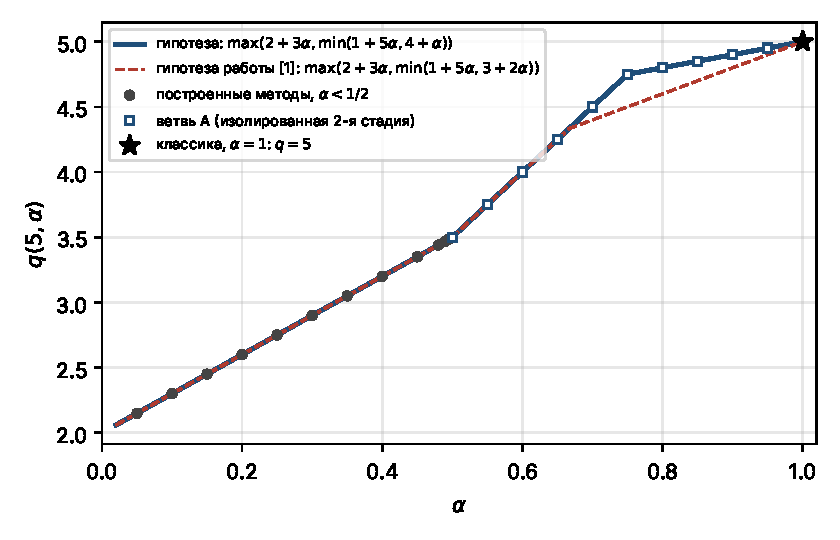
\includegraphics[width=0.7\textwidth]{figs/q5.pdf}
\caption{Барьер для пяти стадий: гипотеза~\ref{conj:q5} (сплошная линия), гипотеза работы~\cite{PrikBarriers} (штриховая), показатели построенных методов (маркеры) и классическое значение при $\alpha=1$.}\label{fig:q5}
\end{figure}

\subsection{Шесть стадий}

Для шести стадий удалось получить лишь нижние оценки. Методы, обнуляющие все условия с показателями ниже указанного уровня, найдены при $\alpha=0.3$ ($q\ge3.2$), $0.4$ ($3.6$), $0.5$ ($4.0$), $0.6$ ($4.6$), $0.7$ ($4.8$), $0.8$ ($5.2$) и $0.9$ ($5.6$). Найти методы с большими показателями не удалось, но с учётом опыта пяти стадий это не может служить даже свидетельством барьера. Естественный следующий шаг~--- построение аналога условий~\eqref{eq:simpl} для шести стадий и соответствующей сокращённой системы.

\section{Выводы}

\begin{enumerate}
\item Для явных методов Рунге--Кутты в форме Вольтерры для уравнений с производной Капуто \emph{доказана} теорема о полном разложении локальной ошибки по корневым деревьям с вершинами двух типов (листья~--- вес $1$, внутренние вершины~--- вес $\alpha$) с явными весами, элементарными дифференциалами и оценкой остатка. Точное решение входит в веса только через квадратурные дефекты висячих вершин.
\item \emph{Доказано}, что во внутренней точке сетки полные производные правой части вдоль решения можно задавать независимо, и, как следствие, условия порядка не только достаточны, но и необходимы (для систем~--- по деревьям, для скалярных уравнений~--- по одночленам). Найдено число условий на каждом уровне.
\item Введены дробные упрощающие условия~\eqref{eq:simpl} и \emph{доказано}, что при пяти стадиях они сводят шестнадцать условий порядка к семи уравнениям на шесть неизвестных, причём один узел остаётся свободным.
\item \emph{Численно установлено}, что сокращённая система имеет при $\alpha\in[0.5;\,0.95]$ два семейства решений, и построены пятистадийные методы с показателем $\min(1+5\alpha,\,4+\alpha)$ и коэффициентами порядка единиц; показатели подтверждены прямым измерением. Тем самым гипотеза работы~\cite{PrikBarriers} о ветви $3+2\alpha$ численно опровергнута и заменена \emph{гипотезой}~\ref{conj:q5}, согласованной с классическим пределом.
\end{enumerate}

Открытыми остаются доказательство гипотезы~\ref{conj:q5} (в том числе полноты решений сокращённой системы), природа зависимости между её уравнениями, перенос упрощающих условий на шесть и более стадий и анализ стартовых шагов, где решение негладкое~\cite{Lubich1983}.

\section*{Благодарности}
Автор выражает глубокую благодарность научному руководителю, члену-корреспонденту РАН И.\,Б.~Петрову за внимание к работе.

\section*{Финансирование работы}
Исследование выполнено за счёт гранта Российского научного фонда № 23-11-00035-П, \url{https://rscf.ru/project/23-11-00035-П/}.

\section*{Конфликт интересов}
Автор данной работы заявляет, что у него нет конфликта интересов.

\begin{thebibliography}{99}\small
\bibitem{PrikBarriers} Приказчиков~Д.\,А. Барьеры порядка явных дробных методов Рунге--Кутты в форме Вольтерры // Ж. вычисл. матем. и матем. физ. (направлена в редакцию).
\bibitem{PP2026zhvm} Приказчиков~Д.\,А., Петров~И.\,Б. Численный метод решения уравнения теории линейной вязкоупругости в слоистых средах // Ж. вычисл. матем. и матем. физ. 2026 (в печати).
\bibitem{Prik2026de} Приказчиков~Д.\,А. Локализация интегродифференциальных уравнений теории линейной вязкоупругости с ядром Работнова // Дифференц. уравнения (направлена в редакцию).
\bibitem{Pouzet1960} Pouzet~P. Méthode d'intégration numérique des équations intégrales et intégro-différentielles du type de Volterra de seconde espèce. Formules de Runge--Kutta // Symposium on the Numerical Treatment of Ordinary Differential Equations, Integral and Integro-Differential Equations (Rome, 1960). Basel: Birkhäuser, 1960. P.~362--368.
\bibitem{BHN1982} Brunner~H., Hairer~E., N{\o}rsett~S.\,P. Runge--Kutta theory for Volterra integral equations of the second kind // Math. Comp. 1982. V.~39, №~159. P.~147--163.
\bibitem{Lubich1983} Lubich~Ch. Runge--Kutta theory for Volterra and Abel integral equations of the second kind // Math. Comp. 1983. V.~41, №~163. P.~87--102.
\bibitem{Garrappa2010} Garrappa~R. Order conditions for Volterra Runge--Kutta methods // Appl. Numer. Math. 2010. V.~60, №~5. P.~561--573.
\bibitem{Butcher1964} Butcher~J.\,C. On Runge--Kutta processes of high order // J. Austral. Math. Soc. 1964. V.~4. P.~179--194.
\bibitem{Butcher2016} Butcher~J.\,C. Numerical Methods for Ordinary Differential Equations. 3rd ed. Chichester: Wiley, 2016.
\bibitem{HNW1993} Hairer~E., N{\o}rsett~S.\,P., Wanner~G. Solving Ordinary Differential Equations I. Nonstiff Problems. 2nd ed. Berlin: Springer, 1993.
\bibitem{repo} Приказчиков~Д.\,А. fractional-vrk-barriers: код и данные. \url{https://github.com/PrikazchikovDA/fractional-vrk-barriers} (ветка \texttt{paper2}).
\end{thebibliography}

\end{document}
